\vspace{-10pt}
\section{Design}
\vspace{-5pt}

FlashMatrix is a matrix-oriented programming framework for machine learning and
statistics.
This work mainly focuses on dense matrices and scales dense matrix operations
beyond memory capacity by utilizing fast I/O devices, such as solid-state drives
(SSDs), in a non-uniform memory architecture (NUMA).

Figure \ref{fig:arch} shows the architecture of FlashMatrix. 
A small number of generalized operations (GenOps)
simplify the implementation and improve expressiveness of
the framework. The optimizer aggressively merges operations to
reduce data movement in the memory hierarchy and achieve better parallelization.
It stores matrices on SSDs through SAFS \cite{safs},
a user-space filesystem for SSD arrays, to fully utilize high I/O
throughput of SSDs.

\begin{figure}
\centering
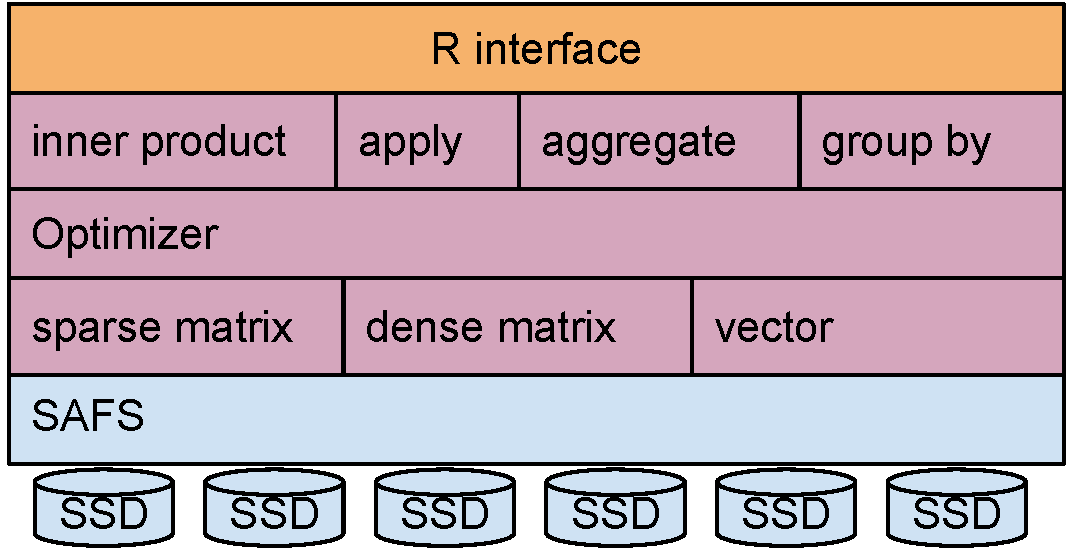
\includegraphics[scale=0.3]{FlashMatrix_figs/architecture.pdf}
\vspace{-2pt}
\caption{The architecture of FlashMatrix}
\label{fig:arch}
\end{figure}

\vspace{-8pt}
\subsection{Programming interface}
\vspace{-4pt}

\begin{table}
\begin{center}
\footnotesize
\begin{tabular}{|l|l|l|}
\hline
GenOp & Description \\
\hline
$C=sapply(A, f)$ & $C_{i,j}=f(A_{i,j})$ \\
\hline
$C=mapply(A, B, f)$ & $C_{i,j}=f(A_{i,j}, B_{i,j})$ \\
\hline
$C=mapply.row(A, B, f)$ & $C_{i,j}=f(A_{i,j}, B_j)$ \\
\hline
$C=mapply.col(A, B, f)$ & $C_{i,j}=f(A_{i,j}, B_i)$ \\
\hline
$c=agg(A, f)$ & $c=f(A_{i,j}, c)$, over all $i$, $j$ \\
\hline
$C=agg.row(A, f)$ & $C_i=f(A_{i,j}, C_i)$, over all $j$ \\
\hline
$C=agg.col(A, f)$ & $C_j=f(A_{i,j}, C_j)$, over all $i$ \\
\hline
%$C=groupby(A, f)$ & $C_k=f(A_{i,j}, C_k)$, where $k$ \\
$C=groupby.row(A, B, f)$ & $C_{k,j}=f(A_{i,j}, C_{k,j})$,\\ & where $B_i=k$, over all $i$ \\
\hline
$C=groupby.col(A, B, f)$ & $C_{i,k}=f(A_{i,j}, C_{i,k})$,\\ & where $B_j=k$, over all $j$ \\
\hline
$C=inner.prod(A, B, f1, f2)$ & $t=f1(A_{i,k}, B_{k,j})$,
\\ & $C_{i,j}=f2(t, C_{i,j})$, over all $k$ \\
\hline
\end{tabular}
\normalsize
\end{center}
\vspace{-12pt}
\caption{Generalized operations (GenOps) in FlashMatrix.
$A$, $B$ and $C$ are matrices, and $c$ is a scalar.}
\label{tbl:genops}
\vspace{-10pt}
\end{table}

FlashMatrix provides a matrix-oriented functional programming interface.
Table \ref{tbl:genops} lists all GenOps, each of which takes matrices and
some functions as input and output new matrices that represent computation results.
The input function defines computation on individual elements in input matrices.
The GenOps can be classified into four categories and each of them represents
a data access pattern: (a) \textit{apply} for
element-wise operations, (b) \textit{agg} for aggregation on a matrix
or on rows/columns, (c) \textit{groupby} for splitting rows/columns
into groups and computing aggregates in each group,
(d) \textit{inner product} for the inner product of two matrices.

The example in Figure \ref{fig:kmeans} computes an iteration of k-means
\cite{kmeans} using GenOps. It first uses \textit{inner.prod} to
compute the Euclidean distance between every data point and every cluster center
and outputs a matrix with each row representing the distances to centers.  
It uses \textit{agg.row} to find the closest
cluster for each data point.  The output matrix 
assigns data points to clusters. It then uses \textit{groupby.row} to count
the number of data points in each cluster and compute the mean of each cluster.

\begin{figure}
\centering
	\footnotesize
	\begin{subfigure}{.25\textwidth}
	\centering
	\begin{minted}[mathescape,
	fontsize=\scriptsize,
	frame=single,
	tabsize=2,
	]{R}
# X is the data matrix.
# C is cluster centers.
kmeans.iter <- function(X,C) {
	# Compute pair-wise distance.
	D<-inner.prod(X,t(C),
			"euclidean","+")
	# Find the closest center.
	I<-agg.row(D,"which.min")
	# Count the number of data
	# points in each cluster.
	one<-rep.int(1,nrow(I))
	CNT<-groupby.row(one,I,"+")
	# Compute the new centers.
	C<-groupby.row(X,I,"+")
	C<-mapply.row(C,CNT,"/")
	list(C=C,I=I)
}
	\end{minted}
  \vspace{-4pt}
	\label{fig:code}
		\caption{R code.}
	\hspace{20pt}
	\end{subfigure}%
	\begin{subfigure}{.25\textwidth}
	\centering
  \vspace{-8pt}
	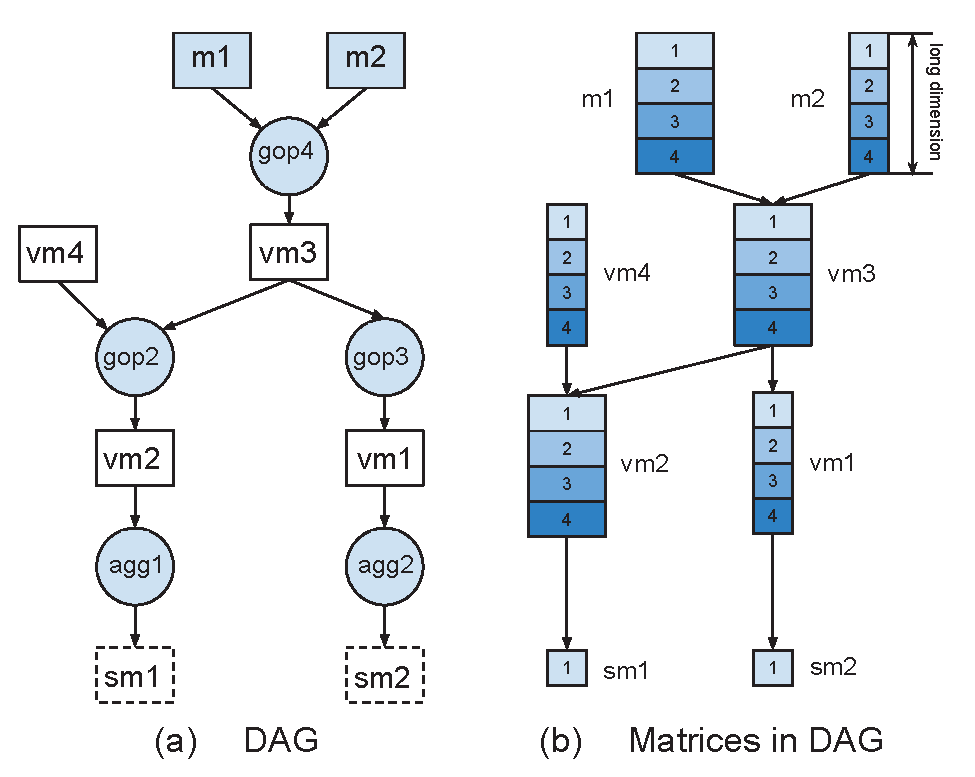
\includegraphics[scale=0.5]{FlashMatrix_figs/DAG.pdf}
	\label{fig:dag}
	\caption{DAG}
	\end{subfigure}
  \vspace{-12pt}
	\caption{k-means implemented with GenOps.}
	\label{fig:kmeans}
  \vspace{-8pt}
\end{figure}

\vspace{-8pt}
\subsection{Dense matrices}
\vspace{-4pt}
FlashMatrix optimizes for matrices that are rectangular because
of their frequent occurence in machine learning and statistics.
Most input data matrices are tall-and-skinny (TAS); they contain
a large number of samples with a relatively few features \cite{}. 
Even if the original data matrices have many features,
the first algorithmic step is usually dimension reduction \cite{}. 
Wide-and-short (WAS) data matrices contain a large number of features with
a few samples \cite{}. Intermediate matrices and output matrices may
be small and square. We store vectors as a one-column dense matrix.
Dense matrices can be stored physically in memory or on SSDs or represented
virtually by a sequence of computations.
We describe FlashMatrix using tall-and-skinny matrices.  We use similar strategies for wide-and-short matrices.

%As such, FlashMatrix optimizes
%for dense matrices that are either tall and skinny or wide and short.   based on their size and shape.
%Our treatment describes the data format for tall matrices.  Wide matrices use similar strategies.

%\subsubsection{Tall-and-skinny matrices} \label{sec:tas_mat}
%\noindent \textbf{Tall-and-skinny (TAS) matrices}:
%FlashMatrix optimizes for \textit{tall-and-skinny} (TAS) dense matrices due to their
%frequent occurrence in data analysis. Many data matrices contain
%a large number of samples with a relatively few features, so data matrices
%are tall and skinny; 

FlashMatrix supports both row-major and column-major
layouts (Figure \ref{fig:den_mat} (a) and (b)).  Supporting both formats
allows FlashMatrix to transpose data without a copy. A TAS matrix is stored
as an SAFS file \cite{safs}.

\begin{figure}
	\centering
	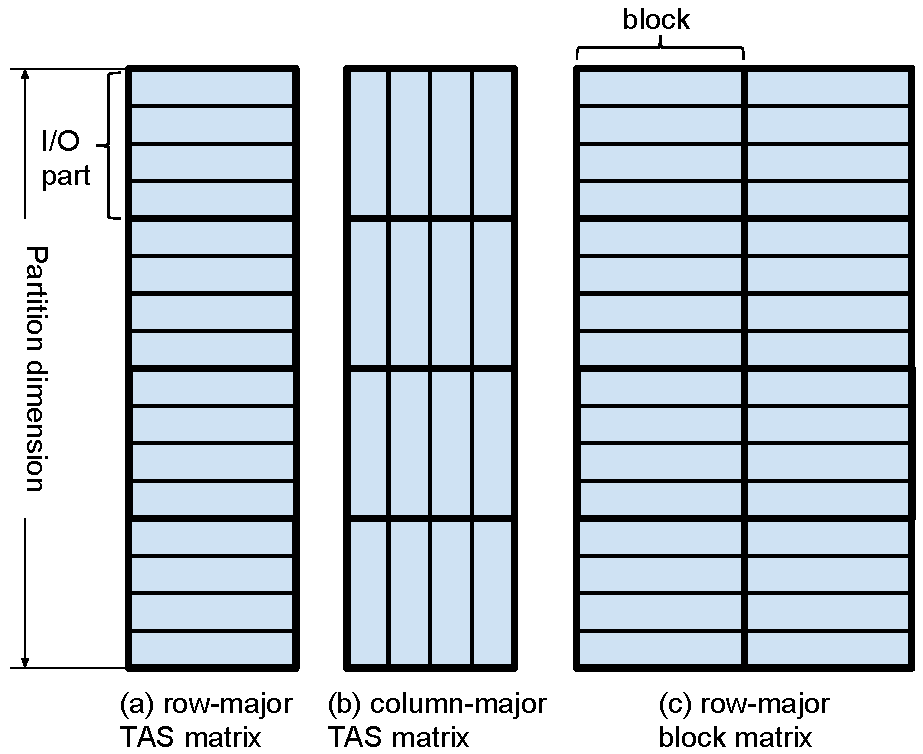
\includegraphics[scale=0.4]{FlashMatrix_figs/dense_matrix2.pdf}
	\caption{The format of a tall dense matrix.}
	\label{fig:den_mat}
  \vspace{-12pt}
\end{figure}

A TAS matrix is partitioned physically into I/O-partitions (Figure
\ref{fig:den_mat}). 
%We refer to the dimension that are partitioned as
%\textit{partition dimension}. 
All elements in an I/O-partition are stored
contiguously regardless of the data layout in the matrix. All 
I/O-partitions have the same number of rows regardless of
the number of columns in a TAS matrix. The number of rows in
an I/O-partition is always $2^i$. This produces column-major TAS
matrices whose data are well aligned in memory to help CPU vectorization.

%\subsubsection{Block matrices} \label{sec:block_mat}
\vspace{3pt}
\noindent \textbf{Block matrices}:
FlashMatrix represents a tall matrix with a group of TAS matrices (Figure
\ref{fig:den_mat} (c)), each with $32$ columns except the last one. We refer
to such a matrix as a \textit{block matrix}. Each of the TAS
matrices is stored as a separate file on SAFS. We decompose a matrix operation
on a block matrix into operations on individual TAS matrices to take advantage
of the optimizations on TAS matrices and reduce data movement.
Coupled with the I/O partitioning on TAS matrices, this strategy enables
2D-partitioning on a dense matrix and each partition fits in main memory.
%\dz{Should we explain GenOps on block matrices in more details?}
%RB maybe -- not sure how to keep it short and clear.

%\subsubsection{Virtual matrices} \label{virt_mat}
\vspace{3pt}
\noindent \textbf{Virtual matrices}:
To support lazy evaluation, FlashMatrix uses \textit{virtual matrices} that
materialize data on the fly during computation and transfer output as input to
the matrix operation. The data of a matrix are not stored physically.
All GenOps output virtual matrices. A GenOp on a \textit{block matrix} may outputs
a block \textit{virtual matrix}. Virtual matrices are assembled to construct
a directed acyclic graph (DAG) that represents a sequence of matrix computations.

\vspace{3pt}
\noindent \textbf{Sink matrices}: Some of the GenOps, such as aggregation and
groupby, output virtual matrices that have a different partition size from
the input matrices. We refer to these virtual matrices as \textit{sink matrices}.
%The GenOps that
%generate \textit{sink matrices} are shown in Table \ref{tbl:sink}.
%In general, \textit{sink matrices} are small and their materialized results
%are always stored in memory. The maximal size of the output matrix from
%an aggregation is $\sqrt{N}$, where $N$ is the number of elements in the input
%matrix. Although the results of groupby and inner product can potentially be
%large, they are small in practice in most of machine learning and data analyis
%tasks because $k$, the number of classes, and $p1$ and $p2$ are usually much
%smaller than the \textit{partition dimension} of a matrix in these tasks.
In general, sink matrices are small and their materialized results are stored
in memory. The maximal size of an output sink matrix from an aggregation
is $\sqrt{N}$ for $N$ elements in the input matrix. The maximal size of
an output sink matrix from a groupby is $k \times \sqrt{N}$ for $k$ classes.
%For most of machine learning and data analysis tasks, 
The output matrix of the inner product of a wide matrix with a tall matrix is usually small because
the long dimension of these matrices is much larger than the short dimension.

% TODO I think we need more formal definition on sink matrices.
%\begin{table}
%\begin{center}
%\footnotesize
%\begin{tabular}{|l|l|l|}
%\hline
%GenOp & Matrix dim & Output size \\
%\hline
%fm.agg & ($n \times p$) & $1$ \\
%\hline
%fm.agg.row & ($n \times p$), $n < p$ & $n$ \\
%\hline
%fm.agg.col & ($n \times p$), $n > p$ & $p$ \\
%\hline
%fm.groupby.row & ($n \times p$), $n > p$ & $p \times k$ \\
%\hline
%fm.groupby.col & ($n \times p$), $n < p$ & $n \times k$ \\
%\hline
%fm.inner.prod & ($p1 \times n$) $\times$ ($n \times p2$), & $p1 \times p2$ \\
%%			  & $n \gg p1, n \gg p2$ &  \\
%\hline
%\end{tabular}
%\normalsize
%\end{center}
%\caption{GenOps that output \textit{sink matrices}.}
%%\label{tbl:sink}
%\end{table}

%In many cases, we do not need to store the data of a matrix physically. Instead,
%we compute and generate its data on the fly. Such matrices are essential for
%lazy evaluation and we refer to these matrices as \textit{virtual matrices}.

%This strategy is essential to reduce data
%movement in the memory hierarchy and memory allocation overhead for creating
%new matrices.

\vspace{-8pt}
\subsection{Reducing data movement}\label{sec:datamove}
\vspace{-4pt}
When evaluating a sequence of matrix operations, FlashMatrix lazily evaluates
GenOps and constructs a DAG automatically because most of the GenOps do not
contain enough computation to achieve in-memory performance. FlashMatrix grows
a DAG as large as possible to increase the ratio of computation to I/O.
Then it performs computation in a DAG all together to minimize data movement
in the memory hierarchy.

Figure \ref{fig:kmeans} (b) shows a DAG for k-means. A DAG comprises a set of
matrix nodes (rectangles)
and computation nodes (ellipses). The majority of matrix nodes are
virtual matrices (dashed line rectangles).
%, which only contains the corresponding matrix operations and input matrices. 
For k-means, only the input matrix \textit{X} has materialized data.
A computation node references a GenOp and input matrices and
may contain some immutable computation state, such as scalar variables and
small matrices needed by the computation. 

To grow a DAG, FlashMatrix allows virtual matrices of different shapes
(Figure \ref{fig:mater}). To simplify evaluation and data flow, 
all virtual matrices in internal matrix nodes need to have the same
\textit{partition dimension}. \textit{Sink matrices} are edge nodes
in the DAG.
%, because
%any computation that uses these \textit{virtual matrices} cannot be connected
%to the same DAG.  

Access to elements of a \textit{sink matrix} triggers materialization of a DAG.
FlashMatrix by default saves only the computation results of sink matrices.
In exceptional cases, especially for iterative algorithms,
FlashMatrix materializes some non-\textit{sink matrices} to avoid
redundant computation and I/O across iterations.  We allow users to
set a flag on non-\textit{sink matrices} to cache the materialized data in memory
or SSDs during computation, similar to caching an RDD in Spark.

\begin{figure}
	\centering
	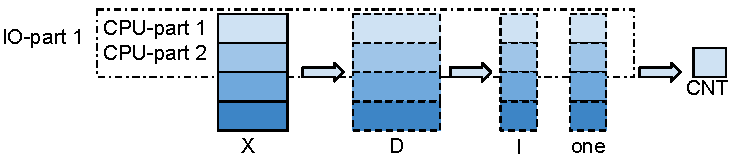
\includegraphics[scale=0.6]{FlashMatrix_figs/materialize.pdf}
  \vspace{-4pt}
	\caption{Materializing matrix partitions in a DAG.}
	\label{fig:mater}
  \vspace{-8pt}
\end{figure}

FlashMatrix partitions matrices in a DAG and
materializes partitions separately (Figure \ref{fig:mater}). This is possible
because all matrices, except sink matrices, share the same partition dimension. 
A partition $i$ of a virtual matrix requires data only from partitions
$i$ of the parent matrices. When a partition is assigned to a thread, it is
processed by the subsequent matrix operations in the same thread to minimize
remote memory access in a NUMA machine.
When materializing a sink matrix, each thread computes partial
aggregation results on the partitions assigned to the thread. 
Then, FlashMatrix merges per-thread partial results to construct the output.

FlashMatrix uses two-level partitioning of dense matrices
to reduce data movement between SSDs and CPU. It assigns I/O-partitions
to a thread as a parallel task.
%A small partition size (\rb{How?}) balances the overhead of accessing a partition,
%computation, skew, and memory consumption. 
It further splits I/O-partitions into Pcache-partitions (processor cache
partitions) at run time and each thread materializes one Pcache-partition
at a time. Matrix operations run on TAS matrices or block matrices that are
divided into TAS matrices so that a Pcache-partition can fit in CPU L1/L2 cache.
Figure \ref{fig:mater} shows recursive materialization of Pcache-partitions.
Matrix \textit{CNT} triggers materialization of
Pcache-partitions of \textit{I} and \textit{one}, which in turn triggers 
partitions of \textit{D}, and so on. Eventually, the process triggers data access
to an I/O-partition of input matrix \textit{X} from SSDs. Upon materializing
output to a virtual matrix, the thread passes the output as input to the subsequent
GenOp, instead of materializing the next Pcache-partition of the virtual matrix
in the same thread. As such, a Pcache-partition still resides in the CPU cache
when the subsequent GenOp consumes
it. This significantly reduces data movement between CPU and memory. In each
thread, all intermediate matrices have only one Pcache-partitions materialized
at any time to reduce CPU cache pollution.
%To reduce CPU cache polution, a CPU-level partition is discarded once it is
%used by all children matrices.
To reduce memory allocation overhead, we recycle memory buffers used for both
I/O and intermediate computation results.

%materialization on block matrices.

%In a DAG, a matrix may be
%required by multiple GenOps. As such, each matrix always buffers one materialized
%CPU-level partition in each thread to avoid redundant computation.

% TODO
%To keep data in CPU cache as long as possible, we reuse the memory buffers
%to reduce the number of memory buffers used in the computation and avoid CPU
%cache polution.

\vspace{-8pt}
\subsection{Parallel execution and I/O access}
\vspace{-4pt}
FlashMatrix dispatches computation to threads so that they
issue large reads and writes to SSDs, while still achieving good load balancing.
FlashMatrix uses a global task scheduler to assign I/O-partitions to threads
dynamically. Initially, the scheduler assigns multiple contiguous I/O-partitions
to a thread. The thread reads these in a single large I/O.
The number of contiguous I/O-partitions assigned to a thread is determined by
the block size of SAFS.
As the computation nears an end, the scheduler dispatches single I/O-partitions. 
The scheduler always ensures that all threads are working on I/O-partitions that are adjacent to
each other on storage.
In this way, if the DAG stores the materialized result of a non-\textit{sink matrix}, 
contiguous regions make it easier for the file system to merge
writes from multiple threads, which helps to sustain write throughout and reduces
write amplification \cite{ripq}.

%For a block matrix with many TAS matrices, we parallelize the computation and
%I/O access differently. One of the goals is to reduce memory consumption.
%Instead of getting the row/column range from all TAS matrices before performing
%computation, we read the row/column range from some TAS matrices first, perform
%computation and move on to the next TAS matrices in the same range. This is
%very helpful if the computation is aggregation.
